\documentclass[12pt]{article}
% REVISION NOTES %%%%%%%%%%%%%%%%%%%%%%%%%%%%%%%%%%%%%%%%%%%%
% 2008-0814 Location, Date, Time
% 2008-0814 fixed citations -- added bibliography.
%
%
\usepackage{geometry}                
\geometry{letterpaper}                   
%\geometry{landscape}                
\usepackage[parfill]{parskip}    
\usepackage{daves,fancyhdr,natbib,graphicx,dcolumn,amsmath,lastpage,url}
\usepackage{amsmath,amssymb,epstopdf,longtable}
\usepackage[final]{pdfpages}
\DeclareGraphicsRule{.tif}{png}{.png}{`convert #1 `dirname #1`/`basename #1 .tif`.png}
\pagestyle{fancy}
\lhead{CE 3305 -- Fluid Mechanics -- SPRING 2024}
\rhead{Name:\_\_\_\_\_\_\_\_\_\_\_\_\_\_\_\_\_\_\_\_\_\_\_\_\_\_\_\_\_\_\_\_\_\_\_\_\_\_\_\_\_\_\_\_}
\lfoot{CE 3305 -- Cleveland}
\cfoot{Page \thepage\ of \pageref{LastPage}}
\rfoot{REVISED: ~12 APR 2024}
\renewcommand\headrulewidth{0pt}
%%%%%%%%%%%%%%%%%%%%%%%%%%%%%%%%%%%%%%%%%%%%%%%%%%%%%%%
\begin{document}
\section*{\center{ { CE 3305 -- Fluid Mechanics} {Exam 3} } }
\section*{Purpose}
Demonstrate ability to apply fluid mechanics and problem solving principles covering topics such as: Dimensional analysis and similitude; turbulent flow in closed conduits; pump system performance.
\section*{Instructions}
\begin{enumerate}
\item Choose any \textbf{four (4)} of the six (6) problems.  You do \textbf{not} need to complete all six problems.
\item Put your name on each sheet you submit.  
\item Use additional sheets as needed. 
\item Begin each problem on a separate page.  Ok to disassemble the exam to keep pages in order.
\item Do not write on the back of sheets (I don't even look)
\item Use the \textbf{problem solving protocol} in the class notes.  The discussion section can simply be the word ``discussion'' 
\item Label and/or underline answers, be sure to include units.
\end{enumerate}
\section*{Allowed Resources}
\begin{enumerate}
\item Your notes
\item Your textbook
\item The mighty Internet with following proviso: \\
 \\ \textbf{You may not communicate with other people during the exam}
\end{enumerate}
\noindent\rule{\linewidth}{0.4pt}
\clearpage

\begin{enumerate}
%%%%%%%%%%%%%%%%%%%%%%%%%%%%%%%%%%%%%%%%%%%%%%%%%%%%%%%%%%%%%%%%%%%%%%%%%%%%%%%%%%%%%%%%%%%%%%%%%%%%%%%%%%%%%%%%%%%%%%%%%%%%%%%%%%%%%
\item A smooth pipe designed to carry crude oil is to be modeled with a smooth pipe 0.75 inches in diameter carrying water (T =60$^o$F ).
The protoype properties are:
\begin{itemize}
\item $D = 47$ inches
\item $\rho= 1.75$ slugs/$ft^3$
\item $\mu=4 \times 10^{-4} ~ \frac{lbf~s}{ft^2}$ 
\end{itemize}
Determine:
\begin{enumerate}
\item  The mean velocity of the water in the model to ensure dynamically similar conditions, if the mean velocity in the prototype is to be 2 ft/s,?
\end{enumerate}
\noindent\rule{\linewidth}{0.4pt}
\clearpage
%%%%%%%%%%%%%%%%%%%%%%%%%%%%%%% SIMILARITY MODELING -- CHEGGable ################################################################
\item Flow around a bridge pier is studied using a $\frac{1}{12}$ scale model.  
The approach velocity in the model is $0.9~\frac{m}{s}$ and at this speed the standing wave at the bridge pier nose is measured to be $2.5~cm$ in height (above the undisturbed water surface).

\begin{figure}[htbp] %  figure placement: here, top, bottom, or page
   \centering
   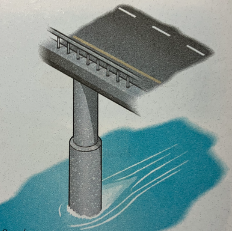
\includegraphics[width=4in]{bridge_pier.png} 
   \caption{}
   \label{fig:bridge_pier}
\end{figure}

Determine:
\begin{enumerate}
\item The approach velocity in the prototype using Froude number matching ($Fr = \frac{V}{\sqrt{gL}}$).
\item The wave height in the prototype.
\end{enumerate}
\noindent\rule{\linewidth}{0.4pt}
\clearpage
%%%%%%%%%%%%%%%%%%%%%%%%%%%%%%% Wenjie Problem %%%%%%%%%%%%%%%%%%%%%%%%%%%%%%%%%%%%%%%%%%%%%
\item A prototype littoral frigate-class vessel has a length of 421 ft and is designed to travel on water at 75 ft/s\footnote{Roughly the specifications of the USS Independence (LCS-2) Littoral Combat Ship}. A 4.21-ft-long model is tested in oil to maintain the same Froude number ($Fr = \frac{V}{\sqrt{gL}}$) and Reynolds number ($Re = \frac{\rho V D}{\mu}$) as the prototype. Determine:
\begin{enumerate}
\item The geometric scaling factor
\item The speed of model ($V_m$) 
\item The required kinematic viscosity of oil ($\nu_m = \frac{\mu_m}{\rho_m}$). 
\end{enumerate}

\noindent\rule{\linewidth}{0.4pt}
\clearpage
%%%%%%%%%%%%%%%%%%%%%%%%%%%%%%%%%%%%%%%%%%%%%%%%%%%%%%%%%%%%%%%%%%%%%%%%%%%%%%%%%%%%%%%%%%%%%%%%%%%%%%%%%%%%%%%%%%%%%
\item In the design of a lift station, a bypass line is often installed parallel to the pump so some liquid recirculates as shown on Figure \ref{fig:pump-bypass}. The bypass valve then controls the flow rate in the system.

\begin{figure}[h!] %  figure placement: here, top, bottom, or page
   \centering
   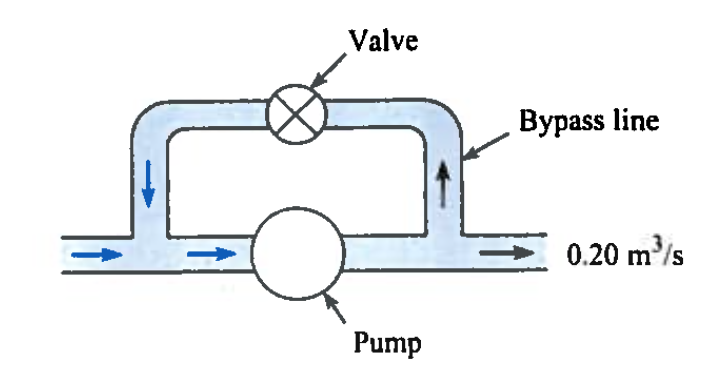
\includegraphics[width=4in]{pump-bypass.png} 
   \caption{}
   \label{fig:pump-bypass}
\end{figure}

The pump performance function is $$h_p = 100 - 100Q$$ where $h_p$ is in meters, and $Q$ is in $\frac{m^3}{sec}$. 
The bypass line is 10~$cm$ in diameter.  The valve setting produces a fitting loss coefficient of $K=0.2$ and this valve loss is the only meaningful head loss at the lift station.  
For a discharge leaving the lift station of 0.2 $\frac{m^3}{sec}$ 

Determine:
\begin{enumerate}
\item The discharge through the pump
\item The discharge through the bypass line
\end{enumerate}

\noindent\rule{\linewidth}{0.4pt}
\clearpage
%%%%%%%%%%%%%%%%%%%%%%%%%%%%%%%%%%%%%%%%%%%%%%%%%%%%%%%%%%%%%%%%%%%%%%%%%%%%%%%%
\item The figure below is a schematic of a pumped-storage system. Water is pumped from the lower reservoir in a pipeline with the following characteristics: D = 300 mm, L = 150 m, $f = 0.029$, $\Sigma K = 5.0$. The radial-flow pump characteristic curve for a single-stage pump is $H_p = 22.9 + 10.7Q -109Q^2$ where $H_p$ is in meters and $Q$ is in $\frac{m^3}{sec}$.

\begin{figure}[h!] %  figure placement: here, top, bottom, or page
   \centering
   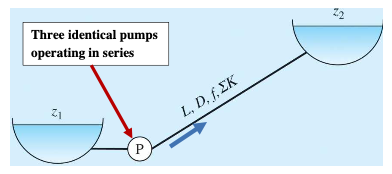
\includegraphics[width=4in]{pss-2.png} 
   \caption{}
   \label{fig:pss-2}
\end{figure}

Determine:
\begin{enumerate}
\item Plot the lift station composite pump curve, and the system curve on the same graph. 
\item The discharge $Q_D$ and pump added head $H_D$ if the lift ($z_2 - z_1$) is 40~$m$ using a three-stage pump (treat as three identical pumps operating in series).
\end{enumerate}

\noindent\rule{\linewidth}{0.4pt}
\clearpage
%%%%%%%%%%%%%%%%%%%%%%%%%%%%%%%%%%%%%%%%%%%%%%%%%%%%%%%%%%%%%%%%%%%%%%%%%%%%%%%%%%%%%%%%%%%%%%%%%%%%%
\item The figure below is a schematic of a parallel pipe system.  Flow occurs from A to B as shown. To augment the flow a pump is located between C and C'. The network is on a plane (flat) surface; all the junction elevations are the same. The pipes are commercial steel.

\begin{figure}[h!] %  figure placement: here, top, bottom, or page
   \centering
   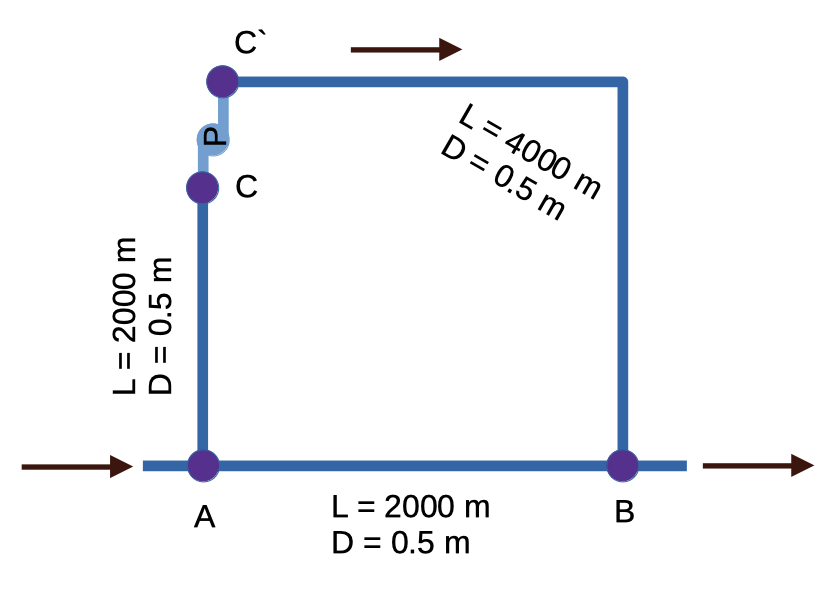
\includegraphics[width=4in]{network-layout.png} 
   \caption{}
   \label{fig:network-layout}
\end{figure}

The pump characteristic curve is shown below:

\begin{figure}[h!] %  figure placement: here, top, bottom, or page
   \centering
   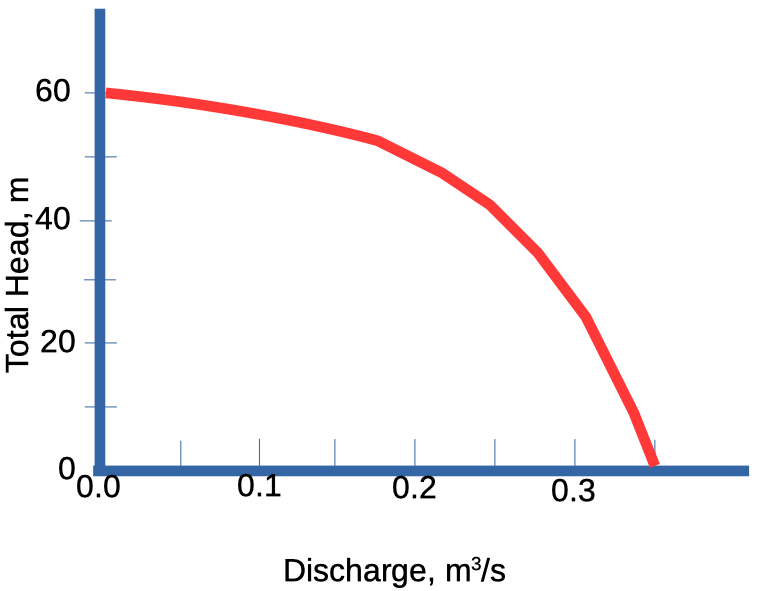
\includegraphics[width=4in]{pump-curve-ex4.png} 
   \caption{}
   \label{fig:pump-curve-ex4}
\end{figure}

Total discharge is 0.60 $\frac{m^3}{sec}$ 

Determine:
\begin{enumerate}
\item The division of flow between pipes A-B and A-C-B
\item The head loss in pipe A-B
\item The head loss in pipe A-C
\item The head loss in pipe C'-B
\item The pump operating conditions.
\end{enumerate}
%%%%%%%%%%%%%%%%%%%%%%%%%%%%%%%%%%%%%%%%%%%%%%%%%%%%%%%%%%%%%%%%%%%%%%%%%%%%%%%%%%%%%%%%%%%%%%%%%%%%%%%%%%

\noindent\rule{\linewidth}{0.4pt}
\clearpage
%%%%%%%%%%%%%%%%%%%%%%%%%%%%%%%%%%%%%%%%%%%%%%%%%%%%%%%%%%%%%%%%%%%%%%%%%%%%%%%%
\end{enumerate}
%%%%%%%%%%%%%%%%%%%%%%%%%%%%%%%%%%%%%%%%%%%%%%%%%%%%%%%%%%%%%%%%%%%%%%%%%%%%%%%%%%%%
\bibliographystyle{chicago}	         % (uses file "chicago.bst")
\end{document}


